\chapter{Classification and regression trees}\label{ch:cart}

\begin{remark}{Outline}
In this chapter, we present a unified framework in which we detail (single)
decision trees methods. In Section~\ref{sec:3:introduction}, we first give an
overview of the context in which these algorithms have been developed. In
Section~\ref{sec:3:tree-structured-models}, we proceed with a mathematical
presentation, introducing all necessary concepts and notations. The general
learning algorithm is then presented in Section~\ref{sec:3:induction} while
more advanced concepts are discussed in finer details in Sections~\ref{sec:3:splitting-rules}
and \ref{sec:3:criteria}. As such, specific algorithms (e.g.,
CART, ID3 or C4.5) are described as specializations of the general framework
presented here.
\end{remark}

\section{Introduction}
\label{sec:3:introduction}

Since always, artificial intelligence has been driven by the ambition to
understand and uncover complex relations in data. That is, to find models that
can not only produce accurate predictions, but also be used to extract
knowledge in an intelligible way. Guided with this twofold objective, research
in machine learning has given rise to extensive bodies works in a myriad of
directions. Among all of them however, tree-based methods stand as one of
the most effective and useful method, capable to produce both reliable and
understandable results, on mostly any kind of data.

Historically, the appearance of \textit{decision trees} is due to
\citet{morgan:1963}, who first proposed a tree-based method called
\textit{automatic interaction dectection} for handling multi-variate
non-additive effects in the context of survey data. Without contest however, the
principal investigators that have driven research on the methodological
principles  are \citet{breiman:1978a,breiman:1978b},
\citet{friedman:1977,friedman:1979} and \citet{quinlan:1979,quinlan:1986} who
simultaneously and independently proposed very close algorithms for the
induction of tree-based models. In particular, the summarizing work of
\citet{breiman:1984}, later complemented with the work of \citet{quinlan:1993},
have set decision trees into a simple and consistent methodological framework,
which largely contributed in making them easy to understand and easy to use by
a large audience.

As we will explore in further details all throughout this work, the success
of decision trees (and by extension, of all tree-based methods) is explained
by several factors that make them attractive in practice:
\begin{itemize}
\item Decision trees are non-parametric. They can model arbitrarily complex relations between inputs and outputs, without any a priori assumption;
\item Decision trees handle heterogeneous data (ordered or categorical variables, or a mix of both);
\item Decision trees intrinsically implement feature selection, making them robust to irrelevant or noisy variables;
\item Decision trees are robust to outliers or errors in labels;
\item Decision trees are easily interpretable, even for non-statistically oriented users.
\end{itemize}

Most importantly, decision trees are at the foundation of
many modern and state-of-the-art algorithms, including forests of randomized
trees (on which this work is about, see Chapter~\ref{ch:forest}) or
boosting methods~\citep{freund:1995,friedman:2001}, where they are used
as building blocks for composing larger models. Understanding all algorithmic
details of single decision trees is therefore an expected prerequisite
for an in-depth analysis of these methods.


\section{Tree structured models}
\label{sec:3:tree-structured-models}

When the output space is a finite set of values, like in classification where
${\cal Y} = \{c_1, c_2, ..., c_J\}$, another way of looking at a supervised
learning problem is to notice that $Y$ defines a partition over the input space ${\cal X}$, that
is
\begin{equation}
{\cal X} = {\cal X}_{c_1} \cup {\cal X}_{c_2} \cup ... \cup {\cal X}_{c_J},
\end{equation}
where ${\cal X}_{c_k}$ is the set of objects $\mathbf{x}$ for which
$Y$ has value $c_k$. Similarly, a classifier $\varphi$ can also be
regarded as a partition of the input space
${\cal X}$ since it defines an approximation $\widehat{Y}$ of $Y$, which in
turn partitions ${\cal X}$, that is
\begin{equation}\label{eqn:3:partition}
{\cal X} = \widehat{{\cal X}_{c_1}} \cup \widehat{{\cal X}_{c_2}} \cup ... \cup \widehat{{\cal X}_{c_J}},
\end{equation}
where
$\widehat{{\cal X}_{c_k}}$ is the set of objects $\mathbf{x}$ such that
$\varphi(\mathbf{x}) = c_k$. Accordingly, learning a classifier can thus
be restated as learning a partition of ${\cal X}$ matching as closely as
possible the (true) partition engendered by $Y$ over ${\cal X}$.

\begin{remark}{Partitioning with noise}
Notice that when $Y$ cannot be univocally de termined given $X=\mathbf{x}$,
e.g., when there is noise on $Y$, then the subsets ${\cal X}_{c_k}$ are not
necessarily disjoints. There may exist couples $(\mathbf{x}_1, y_1)$ and
$(\mathbf{x}_2, y_1)$ such that $\mathbf{x}_1=\mathbf{x}_2$ but $y_1 \neq y_2$.
By contrast, since $\varphi$ defines a function from ${\cal X}$ to ${\cal Y}$,
any input $\mathbf{x} \in {\cal X}$ is mapped to exactly one output $y \in
{\cal Y}$ and the subsets $\widehat{{\cal X}_{c_k}}$ are therefore necessarily
disjoints, which means that no model will ever perfectly predict the true output
value in all cases. As discussed in Section~\ref{sec:2:bayes-model}, this
limitation is unavoidable and can in fact be viewed as the cause of the residual error.
\end{remark}

\subsection{Decision trees}

From a geometrical point of view, the principle of tree structured models is
beautifully simple. It consists in recursively partitioning the input space
${\cal X}$ into subspaces and then assign constant prediction values
$\widehat{y}\in{\cal Y}$ to all objects $\mathbf{x}$ within each terminal
subspace. To make things clearer, let us first define the following concepts:

\begin{definition}
A \emph{tree} is a graph $G=(V,E)$ in which any two vertices (or \emph{nodes})
are connected by exactly one path.
\end{definition}

\begin{definition}
A \emph{rooted tree} is a tree in which one of the nodes has been designated as
the \emph{root}. In our case, we additionally assume that a rooted tree is a
\emph{directed} graph, where all edges are directed away from the root.
\end{definition}

\begin{definition}
If there exists an edge from $t_1$ to $t_2$ (i.e., if $(t_1, t_2)\in E$) then node $t_1$ is said to be the \emph{parent} of
node $t_2$ while node $t_2$ is said to be a \emph{child} of node $t_1$.
\end{definition}

\begin{definition}
In a rooted tree, a node is said to be \emph{internal} if it has one or more
children and \emph{terminal} if it has no children. Terminal nodes are also
known as \emph{leaves}.
\end{definition}

\begin{definition}
A \emph{binary tree} is a rooted tree where all internal nodes exactly
have two children.
\end{definition}

In those terms, a \textit{tree-structured model} (or \textit{decision tree})
can be defined as a model $\varphi: {\cal X} \mapsto {\cal Y}$ represented by a
rooted tree (often binary, but not necessarily), where any node $t$ represents
a subspace ${\cal X}_t \subseteq {\cal X}$ of the intput space, with the root
node corresponding to ${\cal X}$ itself. Internal nodes $t$ are labeled with a
\textit{split} $s_t$ (taken from a set of questions ${\cal Q}$) dividing the
space ${\cal X}_t$ they each represent into disjoint subspaces respectively
corresponding to each of their children. Terminal nodes are labeled with a best
guess value $\widehat{y}_t \in {\cal Y}$ of the output variable. As such, the
predicted output value $\varphi(\mathbf{x})$ for some instance $\mathbf{x}$ is
the label of the leaf reached by the instance when it is propagated through the
tree by following the splits $s_t$.

\begin{figure}
    \centering
    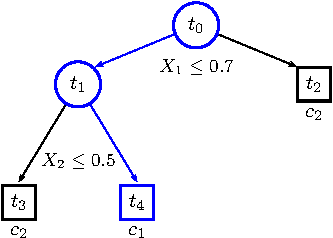
\includegraphics[scale=1.0]{figures/ch3_tree.pdf}
    \caption{A decision tree $\varphi$ built for a binary classification
             problem from an input space ${\cal X}=[0,1]\times[0,1]$.
             (Figure inspired from \citet{breiman:1984}.)}
    \label{fig:3:tree}
\end{figure}

As an example, Figure~\ref{fig:3:tree} illustrates a decision tree $\varphi$
made of five nodes and partitioning the input space ${\cal X} = {\cal X}_1
\times {\cal X}_2 = [0;1] \times [0; 1]$ for a binary classification problem
(${\cal Y}=\{ c_1, c_2 \}$). Node $t_0$ is the root node and corresponds
to whole input space ${\cal X}_0 = {\cal X}$. It is labeled with the split $X_1
\leq 0.7$ which divides ${\cal X}_0$ into two disjoint subsets ${\cal X}_1 \cup
{\cal X}_2$. The first set corresponds to its left child $t_1$ and represents
the set of all input vectors $\mathbf{x} \in {\cal X}_0$ such that $x_1 \leq
0.7$. Similarly, the second set corresponds to its right child $t_2$ and
represents the set of all input vectors $\mathbf{x} \in {\cal X}_0$ such that
$x_1 > 0.7$. Likewise, $t_1$ is labeled with the split $X_2 \leq 0.5$ which
further divides ${\cal X}_1$ into two disjoint subsets ${\cal X}_3 \cup {\cal
X}_4$ respectively corresponding the sets of all input vectors $\mathbf{x} \in
{\cal X}_1$ such that $x_2 \leq 0.5$ (resp. $x_2 > 0.5$). Terminal nodes $t_2$,
$t_3$ and $t_4$ are represented by squares labeled with an output value
$\widehat{y}_t$. They form together a partition (as defined by
Equation~\ref{eqn:3:partition}) of ${\cal X}$, where each set $\widehat{{\cal
X}_{c_k}}$ is obtained from the union of the subspaces ${\cal X}_t$ of all
terminal nodes $t$ such that $\widehat{y}_t = c_k$. In this case,
$\widehat{{\cal X}_{c_1}} = {\cal X}_{t_4}$ while $\widehat{{\cal X}_{c_2}} =
{\cal X}_{t_2} \cup {\cal X}_{t_3}$. As shown in Figure~\ref{fig:3:partition},
the partition engendered by  $\varphi$ on ${\cal X}$ divides the input space
into subspaces that are more and more class homogeneous, starting from ${\cal
X}$ at the root node,  then ${\cal X}_{t_1} \cup {\cal X}_{t_2}$ at the
second level of tree and finally $({\cal X}_{t_3} \cup {\cal X}_{t_4})\cup
{\cal X}_{t_2}$ at the leaves.  As we will explore in
Section~\ref{sec:3:splitting-rules}, the partition is in this case made of rectangles because of
the nature of the splits $s_t$ dividing the nodes. Finally, predictions ...

% , which means that the
% predictions of the decision tree will be correct in most cases, except for a
% few outliers.

\begin{figure}
    \centering
    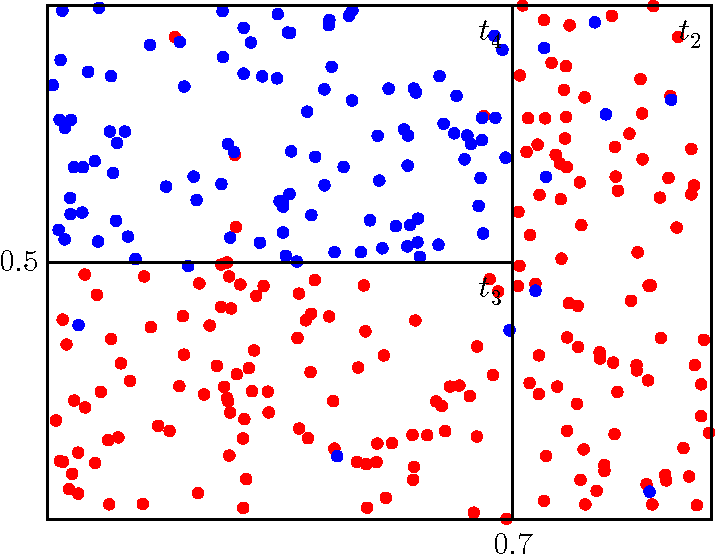
\includegraphics[scale=0.5]{figures/ch3_partition.pdf}
    \caption{Partition of ${\cal X}$ induced by the decision tree $\varphi$.
             Blue dots correspond to objects of class $c_1$ while red dots correspond
             to objects of class $c_2$. (Figure inspired from \citet{breiman:1984}.)}
    \label{fig:3:partition}
\end{figure}





% regression



% \begin{remark}{Notations}
% \end{remark}


%     > définitions formelles + notations
%       + noter que les arbres sont un cas particulier des graphes d'induction
%     > Intuitively, when all variables are ordered, it is like cutting X into rectangles (see CART 31+)
%     > terminal nodes form a partition
% * Prediction

% comment construire l'arbre? choix des splits, d'un critère d'arrêt et des valeurs associées aux feuilles

\subsection{Data structures}

%     > Data structures (arrays vs. object-oriented structures)
%     > definir l'algo de prédiction

\subsection{Example}

%     > (Titanic classification problem) => running example





\section{Induction of decision trees}
\label{sec:3:induction}

% * Growing decision trees
%  Description de l'algo (high-level)
%       * Recursive partition
%           Depth/Breadth/Best first
%       * Splitting rules (overview)
%       * Criterion (overview)
%       * Critères d'arrêts [ différents paramètres, chi² ]
%       * Assignment in terminal nodes

\section{Splitting rules}
\label{sec:3:splitting-rules}

%     > Splitting nodes
%         [ max_features, min_samples_leaf ]
%         - set of questions / answers
%               + categorical vs continuous)
%               + bi-partitions vs n-partitions
%               + weak learners
%         - Best splits
%             + Greedy approximation of optimal trees
%             + optimizing locally the impurity <=> optimizing globally? see page 33+
%         - Approximately best splits
%             + Binning
%             + Subsampling

\section{Goodness of split}
\label{sec:3:criteria}

%     > Impurity criteria
%         - Gini, Entropy, Variance, etc (see cart + graphes)
%         - Efficient implementation for iterative evaluation
%             + How to evaluate multiple candidate thresholds cheaply for
%               a given feature (algorithm, f-ordered)
%             + Sorting algorithms
%         - Effet du critère sur les cuts
%             End-cut preference (CART 11.8)
%             Normalisation par l'entropy (cf. Vincent, Louis)
%             Effet sur la structure des arbres générés
%         - Sample weighting
%             Negative weights? (@ndawe)

% \section{Interpreting decision trees}
% % From trees to rules
